\section{Photography}
The focus of this course are ways of creating images for scientific or medical applications but its worth noting that a majority of all digital images created are digital photography. Digital photography has grown tremendously the last 20 years and analog photography is now limited for some small applications or enthusiast. 

\subsection{Description of digital photography}
Digital photography is an optical imaging technology and the aspects of it are the same as for analogue cameras: Lens quality, aperture, depth of focus and focal length. 

The lenses come in large variety of sized and qualities and it should be chosen with the application in mind. Some basic guidelines are that: bigger is better and glass is better than plastic. Compact lenses has become better and there is a trend towards more compact lenses such as liquid based lenses that can change focal length and focus very rapidly. 

The depth of focus depends on the lens focal length and aperture. A smaller aperture will result in a larger depth of focus but less light is reaching the sensor and therefore need longer exposure time. 

Choosing between a fixed focal length or a zoom lens is depending on the application. For general hobby photography is a zoom lens often to prefer since it doesn't require the user to change lenses when the scene or application changes. Zoom lenses are in general not as good as a fixed lens but instead offer the flexibility. Some geometric distortions to the resulting image is caused by the lens and takes the form of \textbf{Pincushion} or \textbf{Barrel} distortion which can be corrected for in image processing. 

\begin{figure}[ht!]
\centering
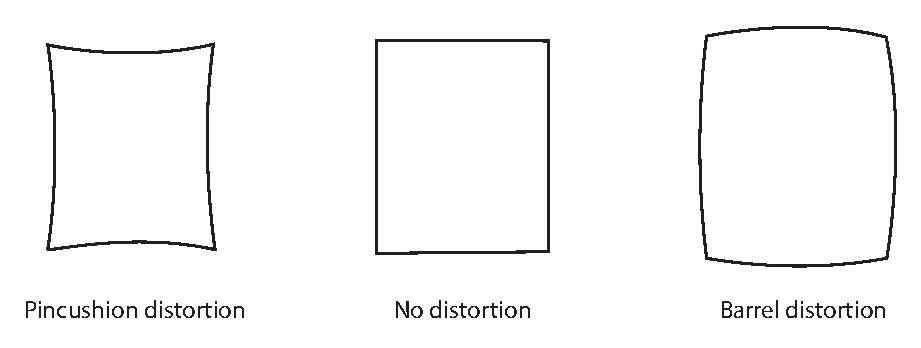
\includegraphics[width=80mm]{figures/distortion.pdf}
\caption{Example of caption}
\label{fig:example}
\end{figure}


There are two types of sensors domination in the area of digital photography: \textbf{CCD} and \textbf{CMOS}. CCD sensors are matrices of photosites each comprised by a photodiode which converts light into a charge and region that can hold the charge. The charges are shifted/moved out of the sensor as a bucket brigade and converted to a digital signal at the end of the circuit. In CMOS sensors similar to the CCD are there photodiodes that converts the light into electrons/ a charge but there is also a reset and select transistor with an amplifier section. This mean that the amplification is done at each pixel. 

In the \textbf{full frame} CCD sensor are the charge holding region integrated with the light sensing region. When the light is collected is happen over the entire imager but it needs to be shut off after that so the charge can be moved through a horizontal charge transfer register a charge voltage conversion, amplifier and analog to digital (A/D) converter. This results in a almost 100\% fill factor of the sensor but there is need for an external shuttering. In the \textbf{interline} type of CCD sensor are the charge holding region shielded from the light meaning there is no need for a external shutter to keep light out. This type of sensor architecture results in lower fill factor but can be compensated with micro-lenses \textcolor{red}{what is that?}. A third type of CCD sensors are \textbf{frame transfer} sensors which have like the \textbf{full frame} photosites that cover almost all of the sensor/sensing area. The difference is that the charges are shifted quickly to a equally sized charge holding region that are shielded from the light. Thanks to the high speed is no shutter need and the readout can be done while a the light for a new image is captured. 

The \textbf{CMOS} sensor is built with the same technique as processors and memory arrays. This architecture allow for readout of the entire array or only parts of it with a simple X-Y address. The fill factor is decreased compared to the full frame CCD since there is more electronic in each pixel. This can be compensated by either Micro-lenses or using thin sensors that can  be exposed from the back side. CMOS sensors can ha

\begin{table}[tb]
 	%\caption{Comparison CCD vs CMOS}
 	\label{tab:tablename}
 	\centering
 
 	\begin{tabular}{ll|c}
 	\hline
 
 	\hline
 	\textbf{CCD} & \textbf{CMOS} \\
 	\hline
 		 Power consumption 2-5W& 				Power consumption 20-50mW  \\
 		 More light sensitive approx 1 lux&	Less light sensitive approx 5 lux \\
 		 Less digital noise& Uses same silicon design as other electronics\\
 		 Better light sensitivity, up to 85\% quantum efficiency& Any subset of pixels can be read out  \\
 		 More color depth, more dynamic range& Younger technology\\
 		 Requires special chips with higher voltage, higher cost& CMOS pushing CCD:s out of the market \\
 	\hline
 	\end{tabular}
 	\caption{Comparison CCD vs CMOS}
 \end{table} 


For a long time have megapixels been a selling point for sensor, the pitch has been: more is better. But this is not always true. A small sensor size with a high number of pixels can lead to decrease in sensitivity and worse signal/noise. 

Comparing priorities between consumer and scientific cameras we can see that consumer cameras generally focus on having good looking pictures while scientific camera priorities correct, quantitative pictures. The increasing use of digital photography has pushed on the development of cameras in the consumer segment, this has also resulted in much value for scientific needs also. Although the trend has now shifted towards smaller sensors since most of them are fitted to mobile phones. This creates a divergence between consumer cameras and scientific cameras that are not faced with the same constraints as mobile phone cameras. As today there is still a wide range of digital cameras for scientific applications. The sensors range from a couple of euros to 10 000 euros in price, but a typical camera can be bought for around 1000 euros. 

A paradigm shift might be taking place with \textbf{Photon counting} sensors being developed. These sensors count each photon separately and is as sensitive as it is possible to be. This allow for new capabilities such as trade off in sensitivity and resolution that can be dependent on the scene. It will allow for motion blur compensation for multiple targets and high apparent SNT for a low photo flux. 

\subsection{Operational steps}
We start of with the lens that most often includes a IR blocking filter and an optical anti-aliasing filter. The focal length is often adjustable (zoom lens) and the focus is controlled by the focus motor. Exposure and focus measuring is done by pressing the shutter button halfway. The lens focuses the light from the scene onto the sensor. The analog signal that is produced by the sensor is then converted to a digital signal (A/D converter). Then the shutter button is fully pressed down the the image is captured and stored on in DRAM. To long exposure times can lead to motion blur in the image which can be solved by active image stabilization, either by moving the lens or the sensor. Exposure control can be used to exposing different parts of the image differently to optimize quality of the image. 


The final high-resolution image is processed by a digital image processor in the camera. The first step is to \textbf{de-mosaicing} since most cameras use the Bayer color filter array, here is interpolation used to fill in the missing color values for each pixel. An algorithm decides if the "missing" color values are in a smooth area or along an edge to determine the value for each missing color value. This process results in a full-color image but not a perfect one. To improve the result there is need for white balancing to compensate for spectral variations in the illumination of the scene. Both daylight from the sun and indoor lightning provides white light is the daylight more "high energy" in the blue portions while indoor lightning is more "high energy" in the red portion of the spectrum. An algorithm is used to analyze the scene and adjust the red and blue signal strength to match the green signal strength in white and neutral parts of the image. Continuing with color correction that is needed since the sensor has a different sensitivity than our eyes and the colors can for the human eye be perceived as unsaturated without correction. The color correction compensate for this and transform the output image to the output color space (often sRGB) that is ready to be displayed on a monitor.  


\subsection{Densitometric}

\subsection{Geometrical}

\subsection{Spectral}

\subsection{Temporal}

\subsection{History}












